\section*{Problem 2}
	\begin{enumerate} [a)]
		\item 
		\begin{proof} [Solution]
			I use the given CA model. Note that the daily infected population is plotted in another scale of second y axis.
			\begin{center}
				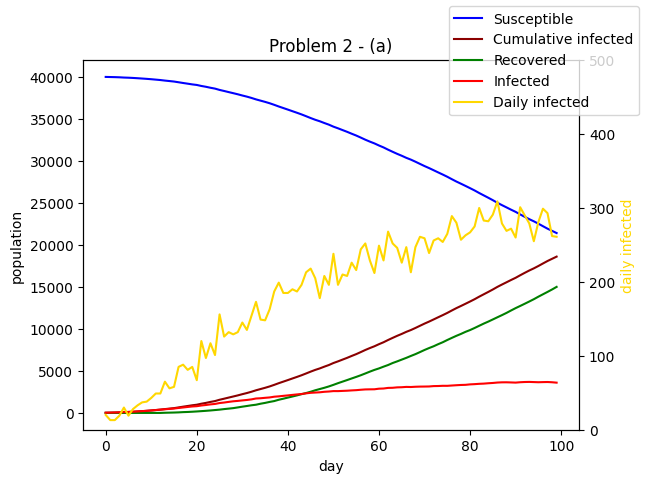
\includegraphics[scale=0.7]{Problem2_a.png}
			\end{center}
		\end{proof}
		\item 
		\begin{proof} [Solution]
			Infection begins at a specific point and spreads randomly from that point. And recovery also follows the flow at certain time intervals. In this model, infection does not occur through other routes, and recovered people are no longer infected. Due to randomness and the impossibility of reinfection after recovery, there may still be uninfected areas even if surrounded by a large yellow area. While it did not spread, a barrier was created for those who have recovered. If both variables were modified, we would expect there to be no such regions.\\
			Domestic infections show similar patterns to the CA model. It can be interpreted that it spread around Seoul and Daegu. However, it does not spread out in a perfectly spherical shape like the model. This is presumed to be due to the existence of additional variables such as transmission distance and infection speed. Therefore, adding these variables to the CA model will allow it to be implemented similar to reality.\\
		\end{proof}
	\end{enumerate}